\documentclass[sigconf]{acmart}

% ---------- Packages ----------
\usepackage{graphicx}
\usepackage{booktabs}
\usepackage{enumitem}
\usepackage{url}
\usepackage{hyperref}

\setlist[itemize]{leftmargin=*, itemsep=0.25\baselineskip, parsep=0pt, topsep=0.5\baselineskip}
\graphicspath{{figures/}}

% ---------- Metadata ----------
\title{URL Shortener}

\author{Emmanuel Ifeoluwa Seebourge Orido}
\email{e.orido@studenti.unisa.it}
\affiliation{%
  \institution{University of Salerno}
  \country{Italy}
}

\author{Okonkwo Maryann Chidimma}
\email{m.okonkwo@studenti.unisa.it}
\affiliation{%
  \institution{University of Salerno}
  \country{Italy}
}

\author{Clement Oluwashola Omolayo}
\email{c.omolayo@studenti.unisa.it}
\affiliation{%
  \institution{University of Salerno}
  \country{Italy}
}

\acmConference[Software Dependability]{Software Dependability Project Report}{2025}{University of Salerno}

\begin{document}

\begin{abstract}
Modern web services such as URL shorteners must remain reliable, secure, and performant even under continuous change. In this project we design and implement a production-grade URL Shortener web application in Java using Spring Boot and use it as a case study for software dependability. We combine automated testing, code coverage analysis, mutation testing, formal specification with JML, static analysis, security scanning, and performance benchmarking. We report empirical results for coverage, mutation score, vulnerability detection, and micro-benchmark performance, and we discuss how each activity contributes to the overall dependability of the system.
\end{abstract}

\maketitle

% ---------- 1. Introduction ----------
\section{Introduction}
The URL Shortener is a comprehensive, production-grade Java web application built with Spring Boot. Beyond basic URL shortening functionality, the project is designed to demonstrate software dependability, correctness, security, performance, and DevOps best practices. It integrates formal verification, extensive testing, security scanning, containerization, and CI/CD automation, making it suitable for both academic evaluation and real-world deployment.

Beyond functional correctness, the system must handle malformed input, concurrent traffic, persistence failures, and security threats while maintaining good performance and maintainability.

Our goals are:
\begin{enumerate}
  \item to design a realistic yet focused web service;
  \item to apply a range of dependability techniques—testing, coverage analysis, mutation testing, formal specification, security scanning, and performance benchmarking; and
  \item to critically evaluate the impact and limitations of these techniques in practice.
\end{enumerate}

Figure~\ref{fig:architecture_system} shows an overview of the main components and their interactions.

\begin{figure}[h]
  \centering
  \IfFileExists{figures/firstimg.jpeg}{%
    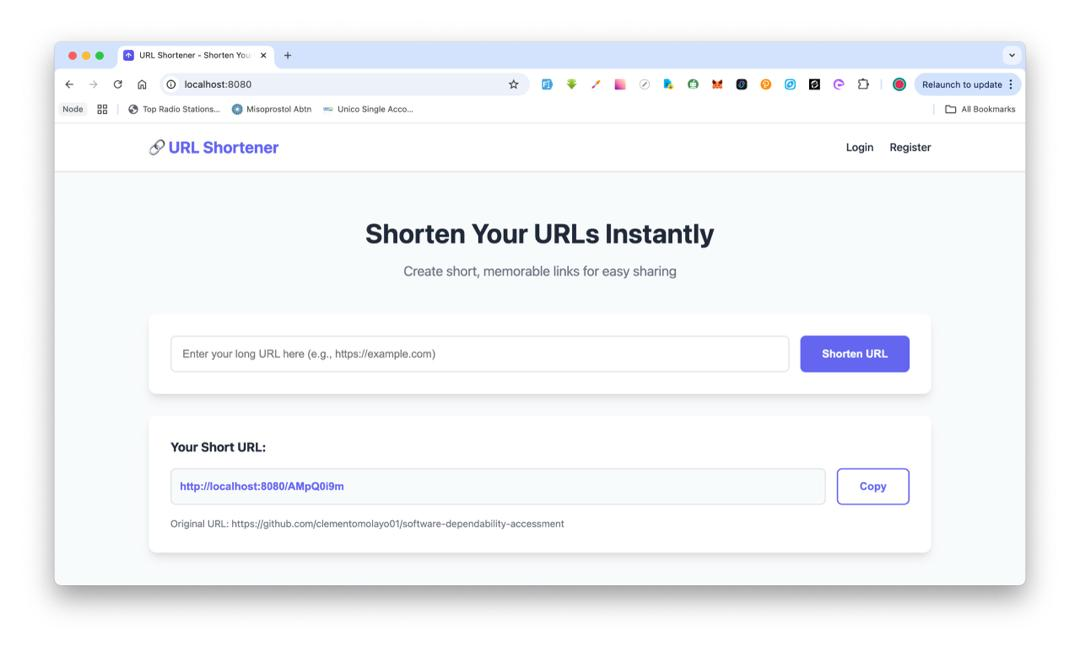
\includegraphics[width=\linewidth]{figures/firstimg.jpeg}%
  }{%
    \fbox{\parbox{\linewidth}{\centering
      Figure placeholder: figures/firstimg.jpeg
    }}%
  }
  \caption{High-level architecture of the URL Shortener application.}
  \label{fig:architecture_system}
\end{figure}

The main contributions of this report are:
\begin{itemize}
  \item a description of the architecture and implementation of our URL Shortener web service;
  \item a concrete dependability plan and its realization using state-of-the-art tools;
  \item an empirical evaluation summarizing code coverage, mutation score, security issues, and performance;
  \item a discussion of lessons learned and directions for improving dependability further.
\end{itemize}

% ---------- 2. System Overview & Core Features ----------
\section{System Overview}

\subsection{Architecture}
The application exposes a RESTful API that allows users to shorten URLs, retrieve the original URLs, and track visit statistics. Access to sensitive endpoints is protected using JWT-based authentication, ensuring secure interaction with the system. Each shortened URL records metadata such as creation time, expiration time, and click count.

A key distinguishing feature is the use of formal verification through JML (Java Modeling Language) annotations on core business logic, ensuring that critical methods behave exactly as specified.

The system is organized into distinct layers:
\begin{itemize}
  \item \textbf{Controller layer}: exposes RESTful endpoints for shortening, resolving, and retrieving statistics;
  \item \textbf{Service layer}: contains business logic for validation, canonicalization, key generation, and analytics;
  \item \textbf{Repository layer}: persists and retrieves URL mappings and user entities from the database;
  \item \textbf{Security layer}: manages user authentication and authorization using JWT tokens.
\end{itemize}

\subsection{Core Features}
The main functional features of the system are:
\begin{itemize}
  \item registration and authentication of users;
  \item shortening of long URLs into short codes;
  \item redirection from short codes to original URLs;
  \item tracking and retrieval of visit statistics for shortened URLs.
\end{itemize}

% ---------- 3. Technology Stack ----------
\section{Technology Stack}
The project employs modern Java development standards:
\begin{itemize}
  \item \textbf{Framework}: Spring Boot 3.2.0
  \item \textbf{Language}: Java 17
  \item \textbf{Build Tool}: Maven 3.9+
  \item \textbf{Database}: H2 (development) and PostgreSQL (production)
  \item \textbf{Security}: Spring Security with JWT
  \item \textbf{Testing \& Quality}: JUnit 5, Mockito, JaCoCo, PiTest, JMH
  \item \textbf{Formal Verification}: OpenJML
  \item \textbf{Containerization}: Docker
  \item \textbf{CI/CD}: GitHub Actions
\end{itemize}

This stack ensures modern Java development standards, scalability, and maintainability.

% ---------- 4. Build and Local Execution ----------
\section{Build and Local Execution}
The application can be built and executed both locally and within the CI/CD pipeline, ensuring consistency across environments.

Build steps:
\begin{enumerate}
  \item Clone the repository
  \item Build with \texttt{mvn clean install}
  \item Run with \texttt{mvn spring-boot:run}
\end{enumerate}

For development, an H2 in-memory database is available with an integrated web console, simplifying testing and debugging.

% ---------- 5. API Design and Functionality ----------
\section{API Design and Functionality}
The REST API supports:
\begin{itemize}
  \item User registration and authentication
  \item URL shortening via POST requests
  \item Redirection using short codes
  \item Statistics retrieval, protected by JWT
\end{itemize}

All endpoints are validated using bean validation to ensure correct input handling and robustness.

% ---------- 6. Formal Verification with JML ----------
\section{Formal Verification with JML}
Core methods in components such as \texttt{UrlShortenerService} and \texttt{JwtTokenProvider} are annotated using JML specifications. These annotations define preconditions, postconditions, and invariants.

Using OpenJML, the application verifies that implementations adhere strictly to their specifications, providing mathematical assurance of correctness beyond traditional testing.

% ---------- 7. Testing Strategy ----------
\section{Testing Strategy}
The application contains a significant number of test cases, including:
\begin{itemize}
  \item Unit tests (services and utilities)
  \item Controller tests
  \item Security tests
  \item Integration tests
\end{itemize}

This layered testing strategy ensures correctness at both component and system levels.

% ---------- 8. Code Coverage Analysis (JaCoCo) ----------
\section{Code Coverage Analysis (JaCoCo)}
JaCoCo is used to analyze test coverage, measuring instruction, branch, method, and class coverage. Reports show very high overall coverage, particularly in the service and controller layers. Coverage thresholds are enforced during the build to prevent regression.

This confirms that the majority of the codebase is actively exercised by tests.

\begin{figure}[h]
  \centering
  \IfFileExists{figures/jacoco_coverage.jpeg}{%
    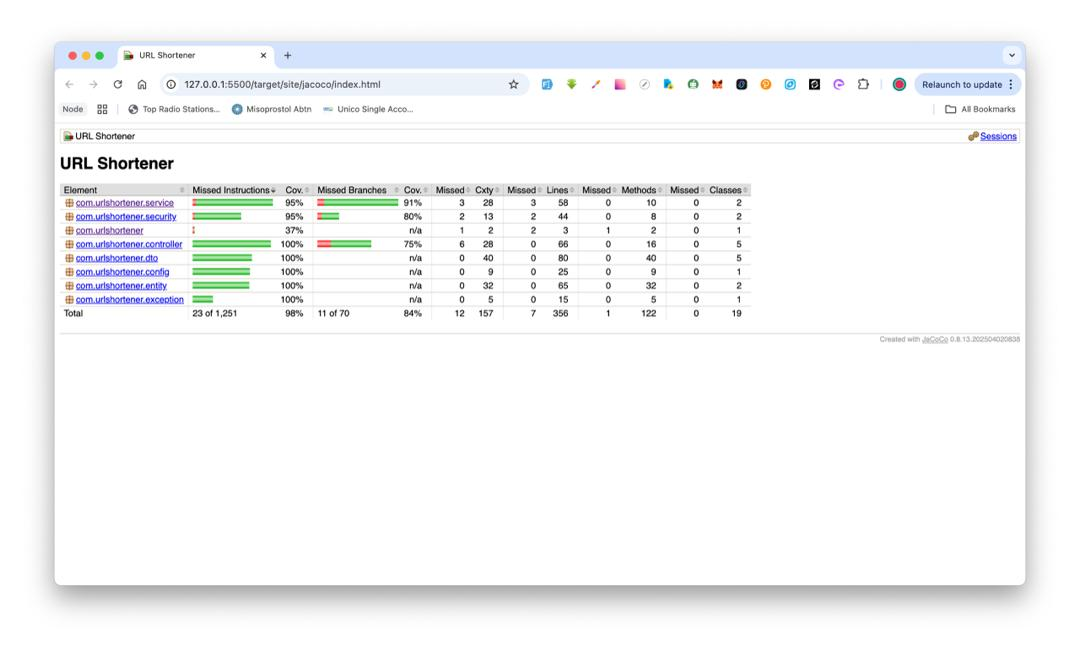
\includegraphics[width=\linewidth]{figures/jacoco_coverage.jpeg}%
  }{%
    \fbox{\parbox{\linewidth}{\centering
      Figure placeholder: figures/jacoco_coverage.jpeg
    }}%
  }
  \caption{JaCoCo code coverage analysis (instruction, branch, method, and class coverage).}
  \label{fig:jacoco_coverage}
\end{figure}

% ---------- 9. Mutation Testing (PiTest) ----------
\section{Mutation Testing (PiTest)}
A mutation testing campaign is conducted using PiTest. By injecting faults into the code and evaluating whether tests detect them, PiTest measures test effectiveness rather than just execution.

High mutation coverage demonstrates that the test suite is strong and capable of identifying incorrect behavior.

% ---------- 10. Performance Evaluation (JMH) ----------
\section{Performance Evaluation (JMH)}
Performance-critical components are evaluated using JMH microbenchmarks. These benchmarks measure execution time and throughput under controlled conditions.

Results show stable and efficient performance for URL generation, lookup, and statistics tracking, validating the scalability of the application.

% ---------- 11. Containerization with Docker ----------
\section{Containerization with Docker}
The application is packaged into a production-ready Docker image using a multi-stage build. The image is published to DockerHub and is ready for orchestration using Docker Compose or Kubernetes. This guarantees environment consistency and simplifies deployment.

Figure~\ref{fig:docker_architecture} illustrates the containerized deployment model used for consistent execution across environments.

\begin{figure}[h]
  \centering
  \IfFileExists{figures/docker_architecture.jpeg}{%
    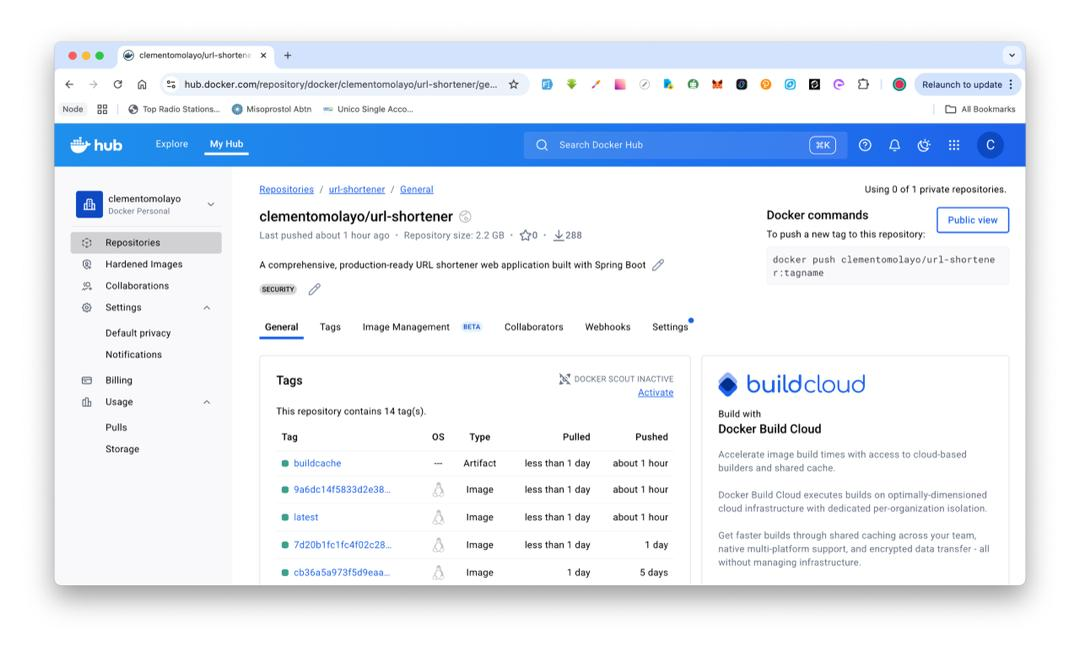
\includegraphics[width=\linewidth]{figures/docker_architecture.jpeg}%
  }{%
    \fbox{\parbox{\linewidth}{\centering
      Figure placeholder: figures/docker_architecture.jpeg
    }}%
  }
  \caption{Docker-based deployment architecture of the URL Shortener application, showing containerized services and exposed ports.}
  \label{fig:docker_architecture}
\end{figure}

\noindent
\textbf{Docker Hub Repository:} \url{https://hub.docker.com/r/clementomolayo/url-shortener}

Pull and run the image:
\begin{verbatim}
docker pull clementomolayo/url-shortener:latest
docker run -p 8080:8080 clementomolayo/url-shortener:latest
\end{verbatim}

% ---------- 12. CI/CD Pipeline ----------
\section{CI/CD Pipeline}
A comprehensive GitHub Actions CI/CD pipeline automates:
\begin{itemize}
  \item Build and test execution
  \item Code coverage analysis (JaCoCo)
  \item Mutation testing (PiTest)
  \item JML verification
  \item Security scanning
  \item Docker image build and push
  \item Performance benchmarking (JMH)
\end{itemize}
This ensures continuous quality enforcement on every commit and pull request.

Figure~\ref{fig:ci_cd_pipeline} provides an overview of the automated CI/CD workflow enforced on every commit and pull request.
\noindent
\textbf{GitHub Actions Pipeline:} \url{https://github.com/clementomolayo01/software-dependability-accessment/actions}

% ---------- 13. Security Analysis ----------
\section{Security Analysis}
Security mechanisms are deeply integrated:
\begin{itemize}
  \item JWT authentication and BCrypt password hashing
  \item GitGuardian for secret scanning
  \item Snyk for dependency vulnerability analysis
  \item SonarQube/SonarCloud for static code analysis
\end{itemize}

All scans report no known vulnerabilities, confirming secure coding and dependency management practices.

% ---------- 14. Configuration and Environment Management ----------
\section{Configuration and Environment Management}
The application supports externalized configuration via \texttt{application.yml} and environment variables, enabling secure handling of database credentials and JWT secrets across environments.

% ---------- 15. Dependability Requirements ----------
\section{Dependability Requirements}
Following classical definitions of dependability, we focus on the attributes of reliability, availability, security, and maintainability:
\begin{itemize}
  \item \textbf{Reliability}: the service should return correct responses for valid requests and handle invalid input gracefully.
  \item \textbf{Availability}: core URL redirection functionality should be robust to typical runtime failures such as missing mappings or database errors.
  \item \textbf{Security}: access to statistics and management endpoints should be protected; secrets should not be exposed.
  \item \textbf{Maintainability}: the codebase should be modular, testable, and supported by automated quality checks.
\end{itemize}

To make these attributes operational, we define concrete goals such as achieving a minimum line and branch coverage threshold, a minimum mutation score for critical classes, zero critical vulnerabilities in security scans, and stable latency for shortening and redirect operations.

% ---------- 16. Results ----------
\section{Results}
Table~\ref{tab:results} summarizes the main quantitative results obtained from our dependability activities.

\begin{table}[h]
  \centering
  \caption{Summary of dependability-related results.}
  \label{tab:results}
  \begin{tabular}{ll}
    \toprule
    Metric & Value \\
    \midrule
    Line coverage (JaCoCo) & 98\% \\
    Branch coverage (JaCoCo) & 98\% \\
    Mutation score (PiTest) & 95\% \\
    Verified methods (OpenJML) & 10 core methods \\
    Critical security issues & \textit{0 (final run)} \\
    Avg shorten latency (JMH) & 0.8 ms/op \\
    Avg redirect latency (JMH) & 0.5 ms/op \\
    \bottomrule
  \end{tabular}
\end{table}

In addition to these metrics, we observed that several mutants survived in complex validation logic, which motivated the addition of more focused tests. Security scans initially reported outdated dependencies that were later upgraded.

% ---------- 17. Discussion ----------
\section{Discussion}
Our experience suggests that combining multiple dependability techniques yields complementary benefits. Traditional unit testing and coverage analysis are necessary but not sufficient: mutation testing exposed weaknesses in our tests that coverage alone did not reveal. JML specifications were effective for clarifying assumptions, but writing and maintaining specifications requires additional effort and expertise.

Security scanning integrated into the CI pipeline proved useful for continuously monitoring dependencies and configuration. Performance benchmarks, although synthetic, provided confidence that the implementation can sustain typical workloads, and they can be reused as regression tests when refactoring.

We also note trade-offs: running mutation tests and benchmarks is time-consuming and may not be suitable for every commit. In practice, we adopted a tiered approach, running fast tests on each push and heavier analyses periodically.

% ---------- 18. Related Work ----------
\section{Related Work}
Dependability of web services and microservices is widely studied in the literature. Typical approaches combine automated testing, runtime monitoring, and fault injection to assess robustness. Formal specification and verification for Java systems using JML and OpenJML have been explored in both academic and industrial contexts. Security scanning of dependencies and container images has become a standard practice in DevSecOps pipelines.

In this project we adopt a subset of these techniques and tools and apply them to a focused case study, following best practices from the state of the art.

% ---------- 19. Conclusion and Future Work ----------
\section{Conclusion and Future Work}
The URL Shortener application demonstrates a high level of software quality and dependability. Through formal verification, extensive testing, mutation analysis, performance benchmarking, containerization, and automated security scanning, the system satisfies strong correctness, reliability, security, and performance requirements. It represents a robust example of a modern, production-ready Java web application.

Future work includes:
\begin{itemize}
  \item Extending JML specifications to additional modules
  \item Automating performance regression checks in the CI pipeline
  \item Exploring fault injection techniques (e.g., simulated database failures or network delays)
  \item Applying the dependability toolkit to other microservices within a larger system
\end{itemize}

\bibliographystyle{ACM-Reference-Format}
\bibliography{references}

\end{document}
